\documentclass[12pt]{article}
\usepackage{hyperref}
\usepackage{graphicx}
\usepackage{array}
\usepackage{tabu}
\usepackage[table]{xcolor}
 

\setlength{\arrayrulewidth}{1mm}
\setlength{\tabcolsep}{18pt}
\renewcommand{\arraystretch}{1.6}
\renewcommand{\today}{September 7 , 2017}


\begin{document}

\begin{titlepage}
	\begin{center}
		
		\LARGE{\textbf{Software Requirements Specification}}
		        
		\vspace{1.5cm}
		      
		\textbf{Glancify} \\
		\small{Version 1.0}
		
					
		\vspace{2cm}
		        
		\large{\textbf{Authors:}}\\
		\large{Neelansh Sahai (201551086)\\
		        Piyush Sikarwal (201551020)
		        }
					
		\vspace{1.5cm}
						
		\large{October  10, 2017}
						
	\end{center}
\end{titlepage}
\newpage
\textbf{Team members :} \\
\begin{center}
	\begin{tabular}{ |m{10em} m{8em} m{9em}|}
		\hline
		TEAM MEMBER        &   & ID        \\
		\hline
		Himanshu Singhal             &   & 201551014 \\
		Piyush Sikarawal          &   & 201551020 \\
		Saurabh Srivastava              &   & 201551032 \\
	    Deepak Sandrana     &   & 201551033 \\
		Sakshee Jain    &   & 201551074 \\
		Neelansh Sahai    &   & 201551086 \\ 
		\hline
	\end{tabular}
	
\end{center}
\newpage
\textbf{Revision History}
\begin{center}
	%\rowcolors{}{white!80!yellow!50}{white!70!white!40}
		\begin{tabular}{ | m{2em} | m{8em} | m{4em} | m{5em} | m{5em} | }
			\hline
			Version & Description                         & Date       & Authors                   & Reviewers           \\
			\hline
			1.0     & First report drafted on Software Requirement Specifications & 4/10/2017  & Neelansh , Piyush & Saurabh, Sakshee , Himanshu , Deepak \\
			\hline
			
		\end{tabular}
    		
	\end{center}
\newpage
\tableofcontents
\newpage

\section{Introduction}
\subsection{Significance of this Document}
Our project mainly aims at improving the lifestyle of all the socially active
users by providing them a user-friendly interface, where they will get a
glance over all the updates related to their social networks. Whether it is
Facebook, Twitter, Quora, Github, etc., our project provides access to all
these social networking platforms.
This document would act as an input to the design phase of the project.
The purpose of this document to serve the project in terms of specifying
the requirements of the project clearly. The need for the project, scope
and various functional and non-functional requirements are described in
detail to ensure that the design phase is carried out with ease and with
clear understanding of the concepts involved.

\subsection{Target Audience for this Document}
This document is intended for developers, testers, users and documentation writers. The Software Requirement Specification is organized into following as Introduction of Project, Overall description, System Specific Requirements and other non-functional requirements.
\par
The reader must go through System Specific Requirements and other non-functional requirements for detailed study of features proposed to be incorporated in project Glancify.

\subsection{Product Scope}
This is the very wide scope project, mainly because there are very few
constraints. Any user who has internet access and is socially active, can
use this product. Also, the fact that social networking platforms are used
all around the globe, the people who belong to the above defined set are
from every corner of the world and thus, the scope of this project covers
a wide range of users.

\subsection{Overview}
The requirement specification captures system requirements for the
following areas:
\begin{itemize}
    \item Functionality
    \item Usability
    \item Reliability
    \item Performance
    \item Supportability
    \item Design Constraints
 
\end{itemize}

\section{Overall Description}

\subsection{What is the Problem?}
The origin of this idea is the fact that, most of the people have accounts
on multiple social networking platforms and, they priorities the events
happening on most of these platforms. Thus, to remain updated to on
their PCs or laptops, the person needs to open these websites, refresh
them again and again, go to the notification panel and scroll through the
notifications. Also suppose, if someone wants to get updates from three
of the social medias, then he will have to open all the three in different
tabs of the browser.

\subsection{Product functions}
\begin{itemize}
    \item Notifications of all the logged in accounts on the new tab page of
the browser, sorted and arranged according its domain.
 
    \item   Providing a “GOTO” button on the bottom of each card to redirect
the user to the respective social networking platform.
 
    \item Providing an “Add” option, to add new cards that will refer to
other social networking accounts. 

\item Providing a “Remove” option, on each card that will remove that
card from the preferences of the user.
\item Providing an option to click on the new tab button (Ctrl + T), and
use the features of the extension.
\end{itemize}

\subsection{Target Audience for the Project}
The target audience for this project will be all the socially active
individuals throughout the globe, who use different kind of social
networking platforms Facebook, Twitter, Quora, Github, etc.

\subsection{Operating Environment}
Software environment:
\begin{itemize}
    \item Google Chrome (focus)
    \item Firefox
    \item Desktop App
\end{itemize}

\subsection{Assumptions and Dependencies}
This is the assumption, that user knows how to add Chrome Extension.

The assumption made here is that, the users use social networking platforms and appreciate remaining updated with their social lives. The user have moderate knowledge of using Internet and
is familiar with using Web Applications.

\subsection{User Documentation}
A short video tutorial will be provided for getting to know the functionality of the system. Apart from this, we also plan to make the user manual available using ReadTheDocs, a VCS enabled documentation generation system. It will allow us to generate documentations in multiple formats on the fly; the formats themselves being PDF, EPUB, Kindle (MOBI), web-based etc.

\subsection{Design and Implementation Constraints}
Our project would be constrained under certain circumstances. These
include:
\begin{itemize}
    \item  The total time available for coding and implementation.

    \item Designing a lightweight UI, so that the extension works properly.
\end{itemize}

\section{External Interface Requirements}
\subsection{User Interface}
Following requirements have been gathered regarding the
interface level design:

\begin{itemize}
    \item The extension should be user friendly. The front-end
part should not be overpopulated with unnecessary
stuff.
    \item For the web app, we will be following material design
conventions.
    \item If an event occurs, the user should be guided with a
message dialog box displaying either the event is successful or an error has occurred.
    \item Flexibility to adjust size of each card in such a
manner that even if there is a single card or there
are multiple cards they all must be visible on the
screen.
    \item Providing a {"}GOTO{"} button on the bottom of each card to redirect
the user to the respective social networking platform. 
\end{itemize}

\subsection{Hardware Interface}
This will be a Chrome Extension so, any hardware which
can run the PC version of Google Chrome above 38.0.0 and
have an internet connection, will be able to run this
extension. In theory the extension will be able to run by all
other devices that can emulate the PC version of Google
Chrome above 38.0.0

\subsection{Software Interface}

\subsection{ Communications Interfaces}
This will be a Chrome extension, but may still link to web
pages. This will be communicating with database server, so
will be making use of the respective social network
database and connecting it to the extension. The primary
forms of communication will be database queries or
requests. The system will need to integrate the extension
for secure login of the different social networks. The
application will need to be synchronized, so that the
information displayed to the user is always up to date.

\section{Functional Requirements}
\subsection{Add}
\begin{itemize}
    \item Description: If a user wants to link a new account with the
extension, then he can click on the add button and go to the
“Select the Media” procedure. 
    \item Priority: High
    \item 
 Stimulus/Response Process:\\
Input: Click on the button\\
Output: "Select the Media" popup.
\end{itemize}

\subsection{Select the Media}
\begin{itemize}
    \item Description: A popup with the list of various social networking
platform.
    \item Priority: High 
    \item Stimulus/Response Process:\\
Input: Select a social networking platform or close the
popup.\\
Output: open the login popup of respective social
networking platform.\\
Process: Show Username and password field.
\end{itemize}

\subsection{Login}
\begin{itemize}
    \item  Description: The users are required to login into their social media
accounts of which they want to add as card on their new tab
page.

    \item Priority: High
    \item Stimulus/Response Process:\\
Input: Respective account username and password.\\
    Output: Displays message if username and
password does not match otherwise adds
the card and shows the notifications.\\

Process: Request through API to login and save the login details to cookies.

 
\end{itemize}

\subsection{Remove}
\begin{itemize}
    \item Description: Removes the card and logs the user out from that
social networking platform.
    \item Priority: High
    \item 
Stimulus/Response Process:\\
Input: Click to remove button.\\
Output: removal of the card and logging out the from the
respective account and readjust the alignment and
orientation of the cards.\\
Process: Request through respective API to log out the
user and remove that card from the new tab page.
\end{itemize}

\subsection{GOTO}
\begin{itemize}
    \item Description: Redirect the user to the corresponding social
networking site.
 
    \item  Priority: High

    \item 
Stimulus/Response Process:\\

Input: Click on the “GOTO” button.\\
Output: Open the corresponding social networking
website on the current tab.\\
Process: Fetch the link of respective social networking
website and requests for that web page. 
\end{itemize}

\subsection{Redirect to webpage by clicking on notifications}
\begin{itemize}
    \item  Description: Redirect the user to the corresponding social
networking site.
    \item  Priority: High
    \item 
 Stimulus/Response Process:\\
Input: Click on any notification.\\
Output: Open the corresponding post to the notification
on social networking website on the current tab.\\
Process: Fetch the link of respective notification and
requests for that web page.
\end{itemize}

\section{Non-functional Requirements}
\subsection{Performance Requirements}
\begin{itemize}
    \item \textbf{User Satisfaction:} The application must be such
that it stands up to the user expectations.
    \item \textbf{Response Time:} The response of all the operation
should be good.
    \item \textbf{Error Handling:} Response to user errors and
undesired situations has been taken care of to
ensure that the application operates without any
uncertainty.
    \item \textbf{User friendliness: }The application is easy to learn
and understand. A naive user can also use the system effectively,
without any difficulties.
\end{itemize}

\subsection{Reliability}
The extension is capable to maintain the specified level of
performance. It will run on all PC version of Google Chrome
above 38.0.0. (Version to be taken care). It’ll be reliable and authenticated by Google.

\subsection{Availability}
Ours is a web based application so generally it will only work if one is connected to the Internet. This will work for Browser extension. The extension will run 24*7 if the internet connection is
available and if Google Chrome is open.

\subsection{Portability}
Since, we are making a Chrome extension. This can be easily used on any operating system like windows, linux, mac os, which support PC version of Google Chrome.

\subsection{Safety Requirement}
As such, there are no safety requirements with this
product, other than any normal hazards of a PC or laptop.
The only hazard is the user using their PCs or laptops for a
long time, which they should not do, as this can affect their
eyesight and other health issues.

\subsection{Security Requirement}
The software should provide a secure login to every
individual user to every single social network, as the user is
providing his/her account’s credentials.
Additionally, the server side is to be regularly maintained
and saved by the malicious attacks. Talking about the physical
security options, the user should himself/herself take care that
no other user uses his/her login account and extract their
personal data.

\subsection{Business Rules}
\subsubsection{User Role}
The user should feel responsible for securing his/her login account from other users.
\subsubsection{Developer Role}
The developer should understand his/her role in creating the application which should not exploit the rights of individuals and should design the software according to these needs of the user and not for any unrelated issues. It’s his duty to understand that the kind of information and the data that is to be associated with the application is important to the users and it must be trusted at the same time.

\section{System Requirement Gathering}
The procedure, we followed to gather system requirements was the survey
through Google Forms. The survey was designed in such a manner that we can
get response from every sector. This helped us greatly in deciding what features
should we implement, what the system should be capable of and, where to
implement them. The survey statistics are discussed in this section.
We have taken the survey which includes the following questions. There were
total of 94 responses for these questions.\\

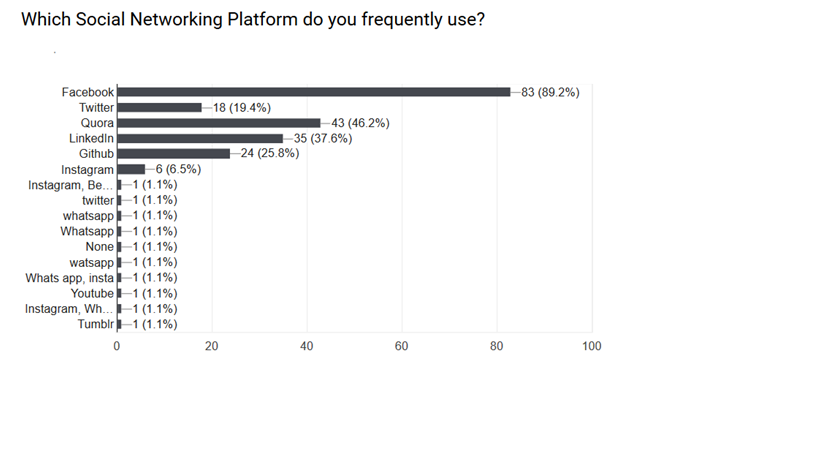
\includegraphics[width=\linewidth]{srs1.png}
  
  
  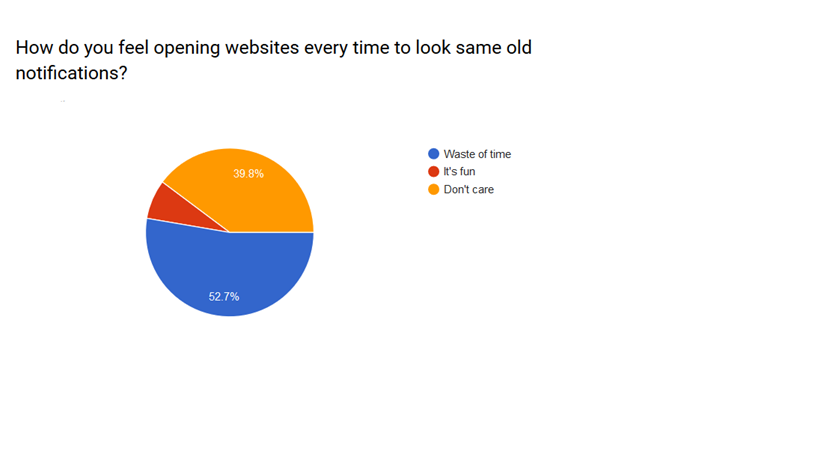
\includegraphics[width=\linewidth]{srs2.png}
  
  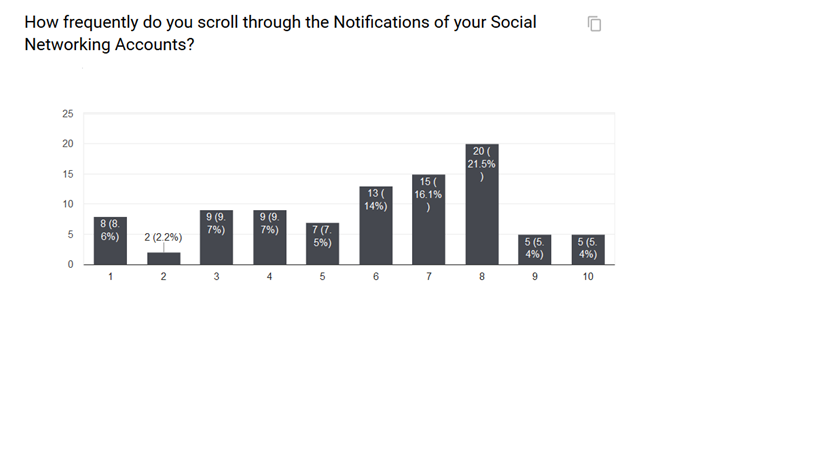
\includegraphics[width=\linewidth]{srs3.png}
  
  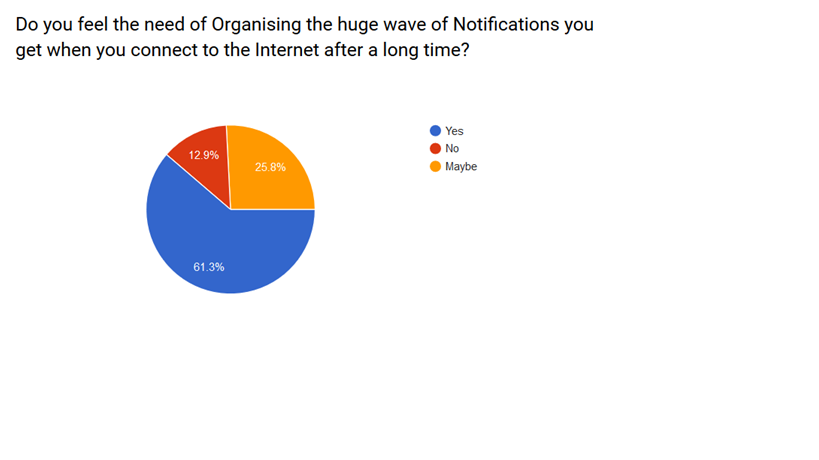
\includegraphics[width=\linewidth]{srs4.png}
  
  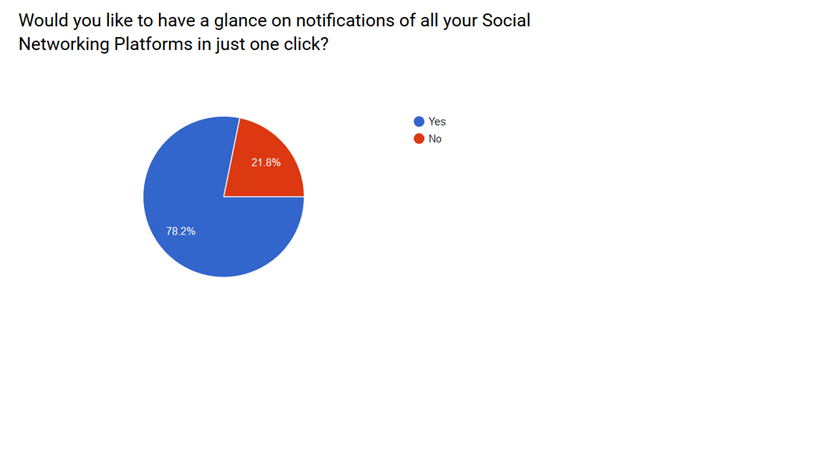
\includegraphics[width=\linewidth]{srs5.png}
  
  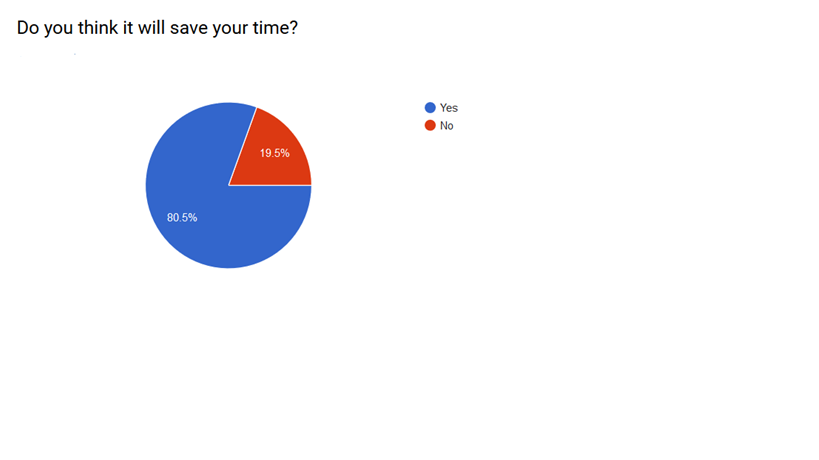
\includegraphics[width=\linewidth]{srs6.png}
  
  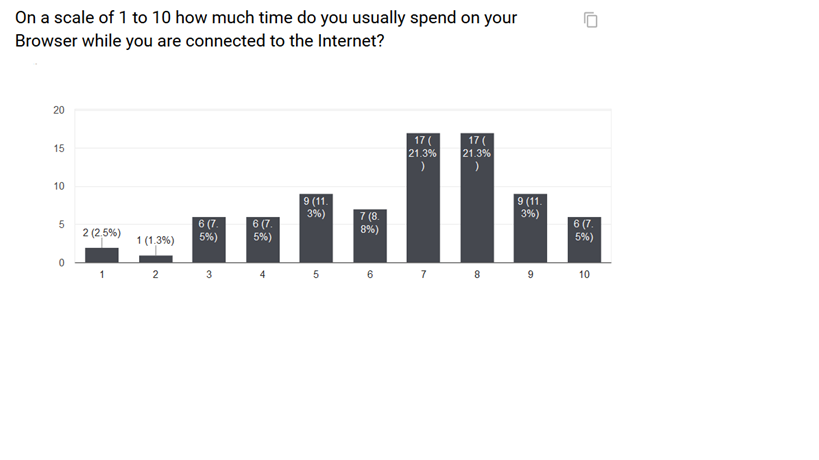
\includegraphics[width=\linewidth]{srs7.png}
  
  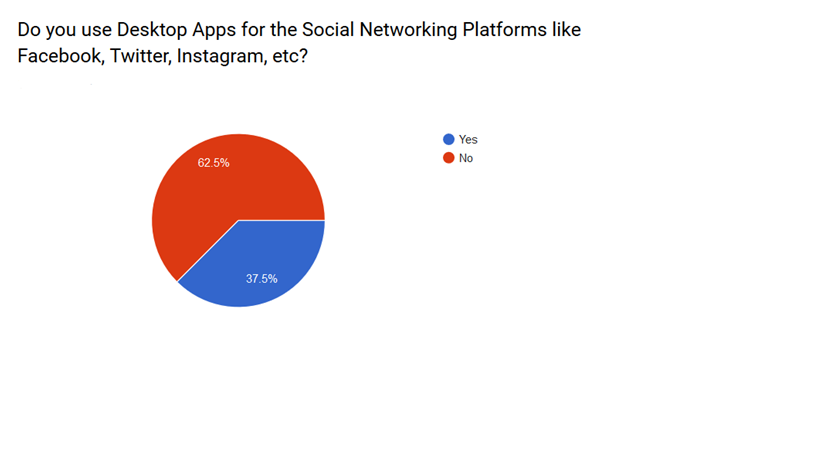
\includegraphics[width=\linewidth]{srs8.png}
  
  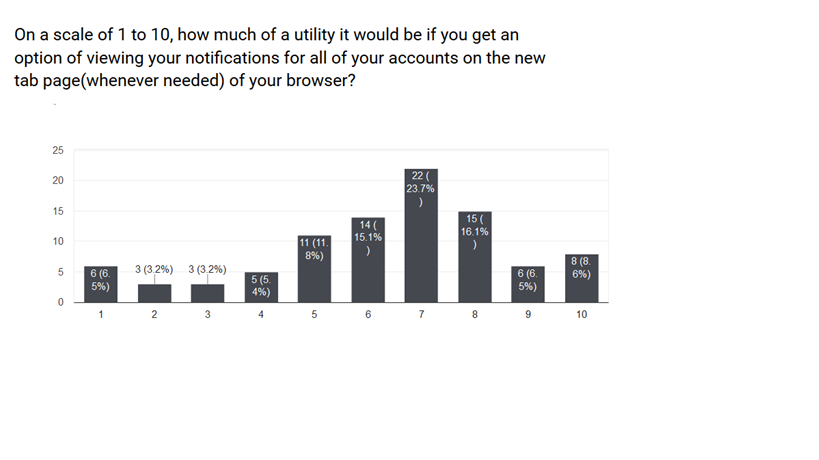
\includegraphics[width=\linewidth]{srs9.png}
  
  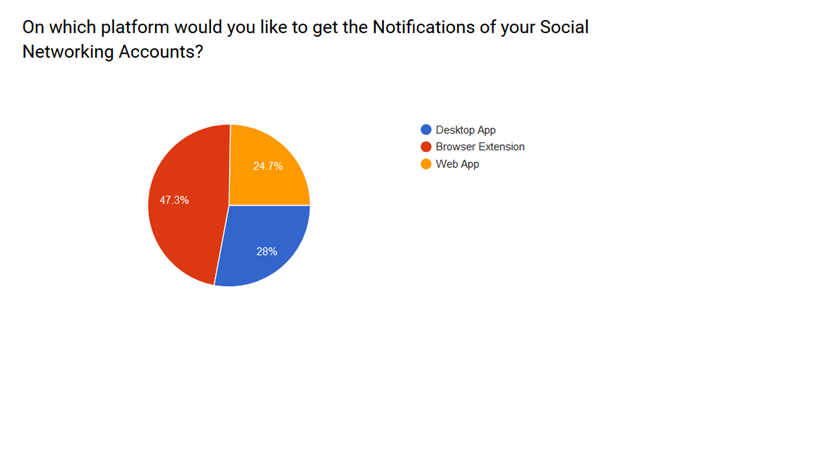
\includegraphics[width=\linewidth]{srs10.png}
  
  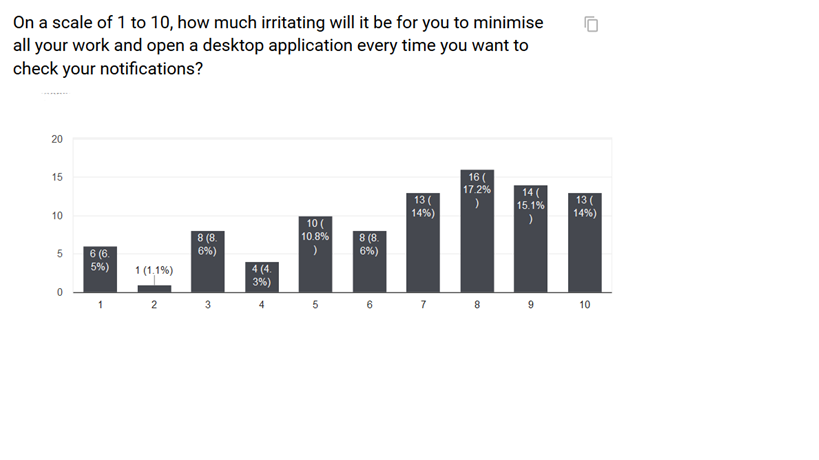
\includegraphics[width=\linewidth]{srs11.png}
  
  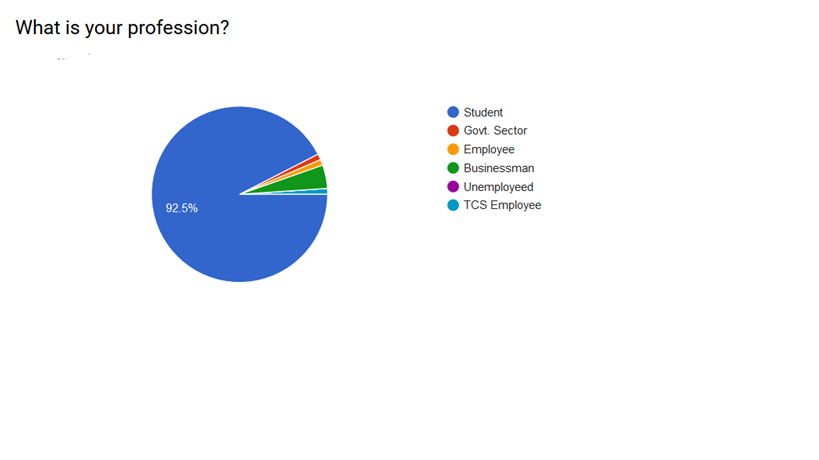
\includegraphics[width=\linewidth]{srs12.png}
  
  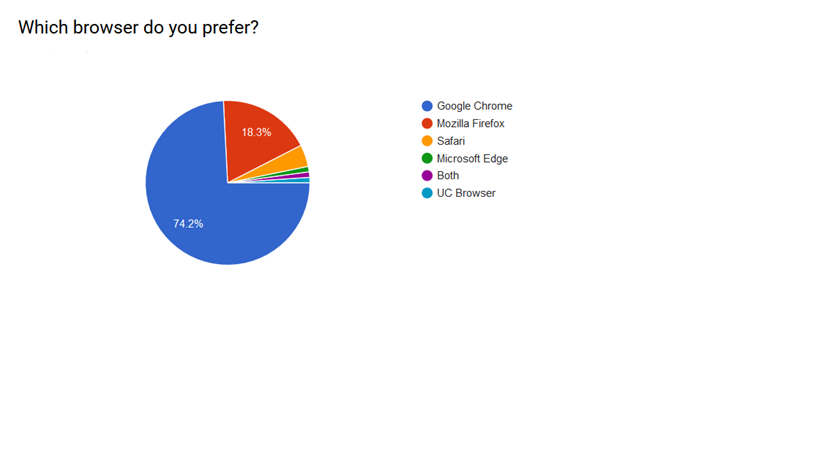
\includegraphics[width=\linewidth]{srs13.png}
  
  
  


\end{document}
